%%=====================================================================
%% SUMÁRIO E INTRODUÇÃO: contexto, problema, objetivos (TCC, cap. 1)
%%=====================================================================
\begin{frame}{Sumário}
  \begin{enumerate}
    \setlength{\itemsep}{0.6em}
    \item Introdução
    \item Fundamentação teórica
    \item Metodologia
    \item Resultados e discussão
    \item Conclusão
  \end{enumerate}
\end{frame}

\secaoudesc{Introdução}

\begin{frame}{Albatroz Aerodesign}
  \begin{columns}[c]
    \begin{column}{0.42\textwidth}
      \begin{itemize}
        \item Competição SAE Brasil Aerodesign
        \item Desde 2022, só motores elétricos sem escovas (BLDC)
        \item O conjunto motopropulsor define a carga útil
      \end{itemize}
    \end{column}
    \begin{column}{0.58\textwidth}
      \centering
      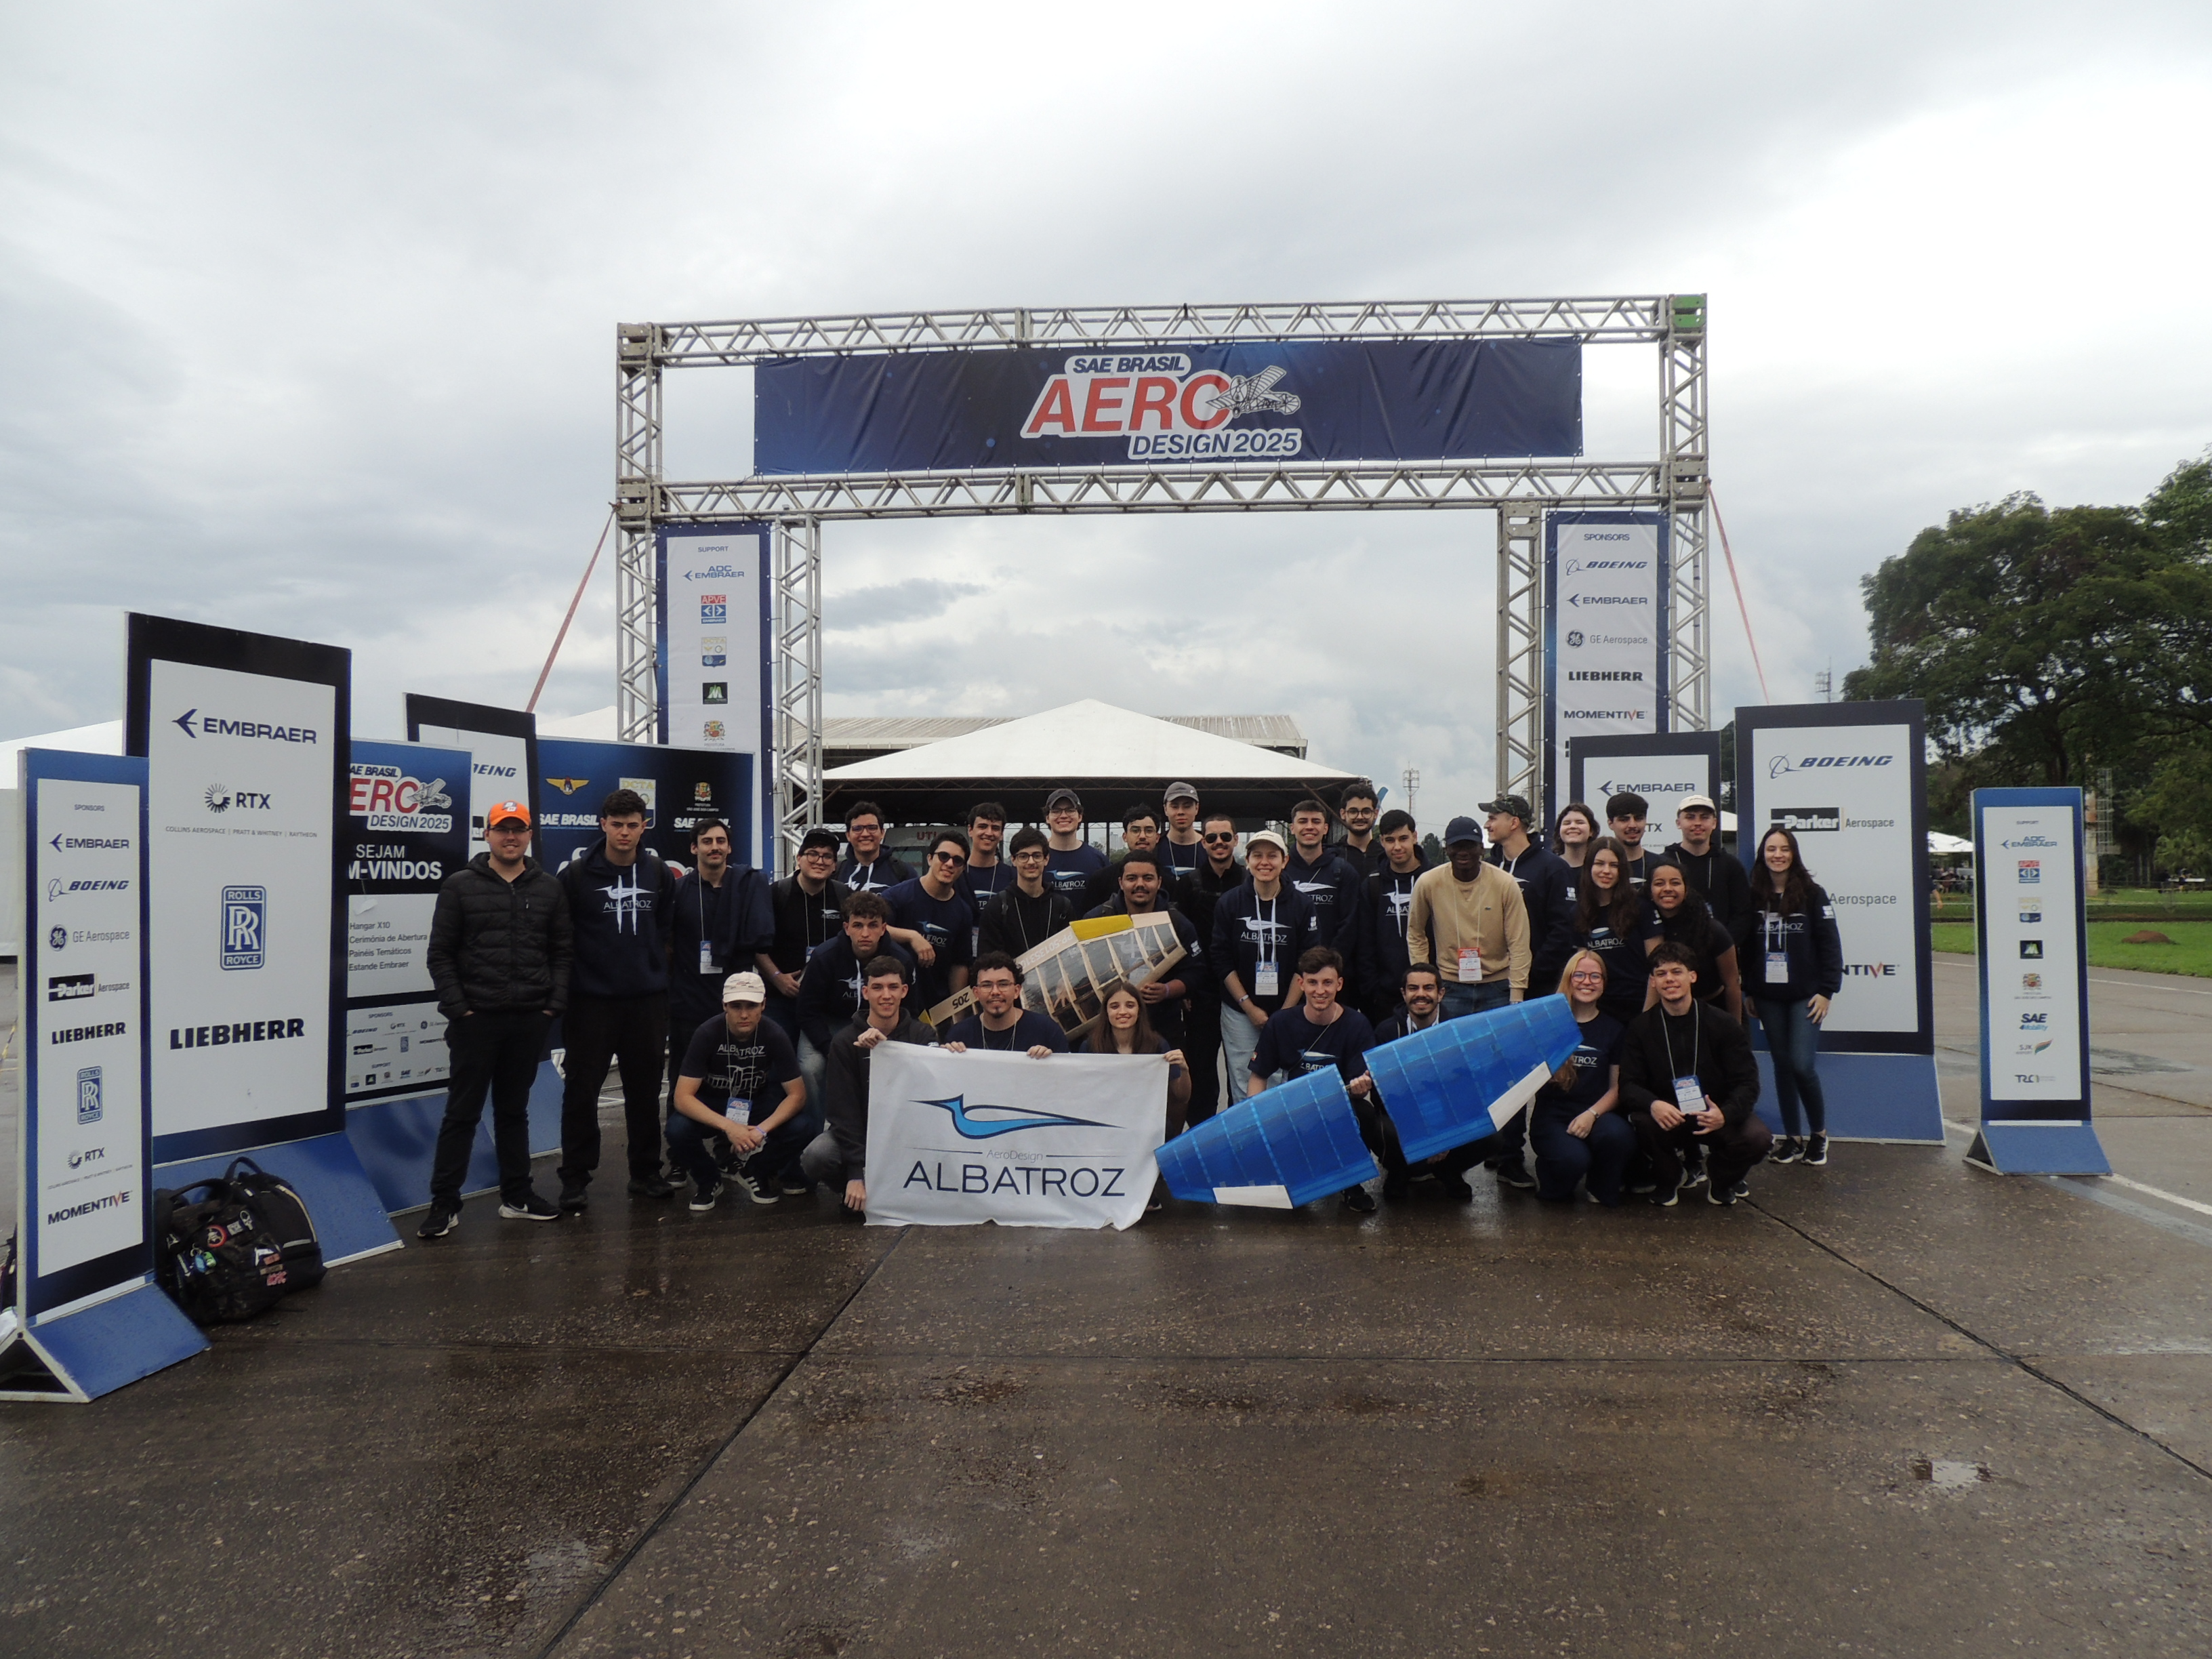
\includegraphics[width=\linewidth]{Introducao/DSCN3474.JPG}
      \fonte[Equipe Albatroz (2025)]
    \end{column}
  \end{columns}
\end{frame}

\begin{frame}{Problema: ensaios fragmentados}
  \centering
  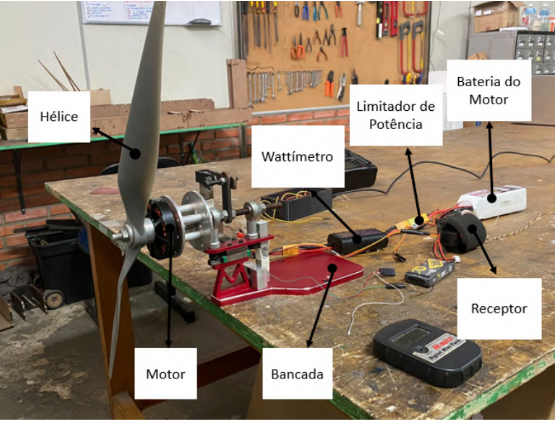
\includegraphics[height=0.6\textheight]{Introducao/BancadaDesempenho.png}
  \fonte[Souza e Veber (2023)]
\end{frame}

\begin{frame}{Objetivos}
  \textbf{Geral:} desenvolver um sistema de aquisição de dados para ensaios de
  conjuntos motopropulsores com motores BLDC.

  \vspace{0.6em}
  \textbf{Específicos:}
  \begin{enumerate}
    \small
    \item Projetar e implementar o sistema de medição do motor (tensão e
          corrente de fase)
    \item Modelar o motor e projetar o observador por modos deslizantes
          (FEM, rotação e torque)
    \item Integrar medição, acionamento e segurança na placa de medição
    \item Interligar placa e supervisório por rede Ethernet (UDP)
    \item Desenvolver o \textit{software} de supervisão em Python
  \end{enumerate}
\end{frame}
